% Copyright 2026 Fausto Spoto
%
% Licensed under the Apache License, Version 2.0 (the "License");
% you may not use this file except in compliance with the License.
% You may obtain a copy of the License at
%
%    http://www.apache.org/licenses/LICENSE-2.0
%
% Unless required by applicable law or agreed to in writing, software
% distributed under the License is distributed on an "AS IS" BASIS,
% WITHOUT WARRANTIES OR CONDITIONS OF ANY KIND, either express or implied.
% See the License for the specific language governing permissions and
% limitations under the License.

\documentclass[11pt]{beamer}  %% versione proiettore
%%\documentclass[11pt,handout]{beamer} %% versione stampa
\usepackage{lucidiJb-2ed}

\usepackage{mathtools}
\usepackage{relsize}
\usepackage{mdframed}
\usepackage[normalem]{ulem}
\usepackage[dvipsnames]{xcolor}
\usepackage{amsmath}
\usepackage{amssymb}
\usepackage{listings, framed}
\usepackage{tikz}
\usetikzlibrary{decorations.pathreplacing}

\mode<article>
{
  \usepackage{fullpage}
  \usepackage{hyperref}
}

\mode<presentation>
{
  \setbeamertemplate{background canvas}[vertical shading][bottom=red!10,top=blue!10]
  \usetheme{Course}
  \usefonttheme[onlysmall]{structurebold}
}

% \|name| or \mathid{name} denotes identifiers and slots in formulas
\def\|#1|{\mathid{#1}}
\newcommand{\mathid}[1]{\ensuremath{\mathit{#1}}}
% \<name> or \codeid{name} denotes computer code identifiers
\def\codesize{\small}
\def\<#1>{\codeid{#1}}
\newcommand{\codeid}[1]{\ifmmode{\mbox{\codesize\ttfamily{#1}}}\else{\codesize\ttfamily #1}\fi}

\newcommand{\todo}[1]{{\color{red}\bfseries [[#1]]}}
\newcommand{\wrt}{\textit{wrt.\ }}
\newcommand{\st}{\textit{s.t.\ }}
\newcommand{\ie}{, \textit{ie.}, }
\newcommand{\ieinitial}{\textit{ie.}, }

\newcommand{\lvalue}{\|lvalue|}
\renewcommand{\exp}{\|exp|}
\newcommand{\com}{\|com|}
\newcommand{\aop}[2]{{#1}\ \mathit{aop}\ {#2}}
\newcommand{\cop}[2]{{#1}\ \mathit{cop}\ {#2}}
\newcommand{\negcop}[2]{{#1}\ \neg\mathit{cop}\ {#2}}
\newcommand{\copfull}[3]{{#1}\ \mathit{#2}\ {#3}}
\newcommand{\field}[2]{{#1}\mathtt{.}{\mathit{#2}}}
\newcommand{\listread}[2]{{#1}[{#2}]}
\newcommand{\size}[1]{{#1}\mathtt{.size()}}
\newcommand{\random}[1]{\mathtt{random(}{#1}\mathtt{)}}
\newcommand{\last}[1]{{#1}\mathtt{.last()}}
\newcommand{\new}[2]{\mathtt{new}\ \mathit{#1}\mathtt{(}{#2}\mathtt{)}}
\newcommand{\call}[3]{{#1}\mathtt{.}{#2}\mathtt{(}{#3}\mathtt{)}}
\newcommand{\push}[2]{{#1}\mathtt{.push(}{#2}\mathtt{)}}
\newcommand{\receive}[2]{{#1}\mathtt{.receive(}{#2}\mathtt{)}}
\newcommand{\require}[2]{\mathtt{require(}\cop{#1}{#2}\mathtt{)}}
\newcommand{\assign}[2]{{#1}\mathtt{:=}{#2}}
\newcommand{\nop}{\mathtt{nop}}
\newcommand{\return}{\mathtt{return}}
\newcommand{\ife}[4]{\mathtt{if\ (}{#1}\ \mathit{cop}\ {#2}\mathtt{)\ then\ }{#3}\mathtt{\ else\ }{#4}}
\newcommand{\ifetwo}[4]{\begin{array}{l}
    \mathtt{if\ (}{#1}\ \mathit{cop}\ {#2}\mathtt{)}\\
    \mathtt{\ then\ }{#3}\mathtt{\ else\ }{#4}
\end{array}}
\newcommand{\for}[3]{\mathtt{for\ }{#1}\mathtt{\ in\ }{#2}\ {#3}}
\newcommand{\sequence}[2]{{#1}\mathtt{;}{#2}}
\newcommand{\bo}{{\mathbb{BO}}}
\newcommand{\boderivation}{\vdash_\bo}
\newcommand{\LValue}{\mathsf{LValue}}
\newcommand{\Exp}{\mathsf{Exp}}
\newcommand{\Com}{\mathsf{Com}}
\newcommand{\Var}{\mathsf{Var}}
\newcommand{\PP}{\mathsf{PP}}
\newcommand{\dastates}[1]{\mathsf{DA}_{{#1}}}
\newcommand{\paths}{\mathsf{P}}
\newcommand{\sideeffect}[1]{\mathsf{se}\left({#1}\right)}
\newcommand{\intsideeffect}{I_{\mathsf{se}}}
\newcommand{\dom}{\mathit{dom}}
\newcommand{\pair}[2]{\langle{#1},{#2}\rangle}
\newcommand{\unchanged}{\mathit{unchanged}}
\newcommand{\survives}[1]{\xrightarrow{{#1}}}
\newcommand{\nat}{\mathbb{N}}
\newcommand{\res}{\mathit{res}}
\newcommand{\val}{\mathit{value}}
\newcommand{\length}{\mathit{len}}

% invariants inside the code
\newcommand{\invariant}[1]{\color{magenta}{#1}}

\subtitle{Deuxi\`eme Colloque International Interreg\\Antananarivo, Madagascar, 3/11/2026}
\title{Boundedness Analysis of Smart Contracts}
\institute{Universit\`a di Verona/Universit\'e de la R\'eunion}
\date{3/11/2026}

\setbeamercovered{invisible}

\AtBeginSection[]{
  \begin{frame}
  \vfill
  \centering
  \begin{beamercolorbox}[sep=8pt,center,shadow=true,rounded=true]{title}
    \usebeamerfont{title}\insertsectionhead\par%
  \end{beamercolorbox}
  \vfill
  \end{frame}
}

\def\setallcolors{%
  \gdef\mybasiccolor{\color{black}}%
  \gdef\mykeywordcolorone{\color{blue}}%
  \gdef\mykeywordcolortwo{\color{teal}}%
  \gdef\mykeywordcolorthree{\color{violet}}%
  \gdef\mykeywordcolorfour{\color{red}}%
  \gdef\mycommentcolor{\color{gray}}%
  \gdef\mystringcolor{\color{red}}%
  \gdef\myidentifiercolor{\color{black}}%
}
\def\setallgray{%
  \gdef\mybasiccolor{\color{lightgray}}%
  \gdef\mykeywordcolorone{\color{lightgray}}%
  \gdef\mykeywordcolortwo{\color{lightgray}}%
  \gdef\mykeywordcolorthree{\color{lightgray}}%
  \gdef\mykeywordcolorfour{\color{lightgray}}%
  \gdef\mycommentcolor{\color{lightgray}}%
  \gdef\mystringcolor{\color{lightgray}}%
  \gdef\myidentifiercolor{\color{lightgray}}%
}

\setallcolors

\lstdefinelanguage{pseudo}{
        keywords=[1]{assert, break, case, catch, class, final, continue, default, do, else, extends, false, finally, for, if, implements, import, instanceof, interface, new, private, 
protected, public, static, payable, return, super, switch, this, throw, throws, true, try, var, while,in },
        keywordstyle=[1]\mykeywordcolorone\bfseries,
        keywords=[2]{Contract, PayableContract, List, int, float, double, short, byte, long, boolean, void, String},
        keywordstyle=[2]\mykeywordcolortwo\bfseries,
        keywords=[3]{this, caller, amount, now},
        keywordstyle=[3]\mykeywordcolorthree\bfseries,
        keywords=[4]{push, require, receive, size, random},
        keywordstyle=[4]\mykeywordcolorfour\bfseries,
        identifierstyle=\myidentifiercolor,
        sensitive=true,
        comment=[l]{//},
        morecomment=[s]{/*}{*/},
        commentstyle=\mycomentcolor\ttfamily,
        stringstyle=\mystringcolor\ttfamily,
        basicstyle=\mybasiccolor\scriptsize\ttfamily,
        morestring=[b]',
        morestring=[b]"
}

\newcommand{\CodeSymbol}[1]{\mybasiccolor{#1}}   % Code associated to defining styles

\lstset{ % define general preferences
        language=pseudo,
        %backgroundcolor=\color{verylightgray},
        extendedchars=true,
        showstringspaces=false,
        showspaces=false,
        numbers=left,
        numberstyle=\scriptsize,
        numbersep=5pt,
        tabsize=2,
        breaklines=true,
        showtabs=false,
        captionpos=b,
        literate={\{}{{\CodeSymbol{\{}}}1
           {\}}{{\CodeSymbol{\}}}}1
           {(}{{\CodeSymbol{(}}}1
           {.}{{\CodeSymbol{.}}}1
           {~)}{{\CodeSymbol{)}}}1
           {>}{{\CodeSymbol{$>$}}}1
           {<}{{\CodeSymbol{$<$}}}1
           {=}{{\CodeSymbol{$=$}}}1
           {;}{{\CodeSymbol{$;$}}}1,
        escapeinside={||},
}

\begin{document}

\begin{frame}
  \titlepage
\end{frame}

\begin{frame}{Smart contracts live in the wild}

  \begin{center}
    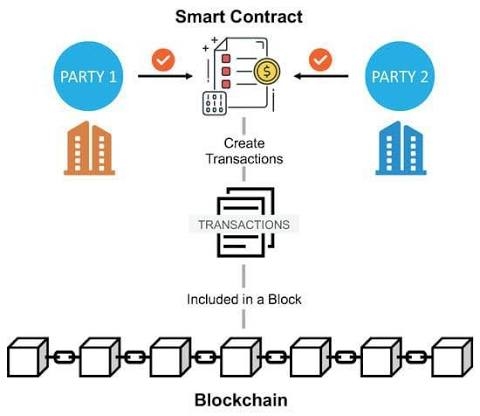
\includegraphics[width=.7\textwidth]{pictures/smart-contract}
  \end{center}

\end{frame}

\begin{frame}[fragile]{Example: a gradual Ponzi scheme}

  \begin{center}
    \begin{minipage}{0.95\textwidth}
      \begin{lstlisting}[language=pseudo]
public class Ponzi1 extends Contract {
  private final List<Contract> investors;
  private int minimum_investment;

  public Ponzi1() {
    investors = new List();
    investors.push(caller);
    minimum_investment = 1000;
  }

  public payable void invest() {
    require(amount >= minimum_investment, "too little");

    int eachInvestorGets = amount / investors.size();
    for investor in investors
      investor.receive(eachInvestorGets);

    investors.push(caller);
    minimum_investment = amount * 11 / 10;
  }
}
      \end{lstlisting}
    \end{minipage}
  \end{center}
  
\end{frame}

{\clearpage
\addtocounter{framenumber}{-1}
\begin{frame}[fragile]{Example: a gradual Ponzi scheme}

  \begin{center}
    \begin{minipage}{0.95\textwidth}
      \begin{lstlisting}[language=pseudo,numbers=none]
|\setallgray|public class Ponzi1 extends Contract {
  |\setallcolors|private final List<Contract> investors;
  |\setallgray|private int minimum_investment;

  |\setallcolors|public |\setallgray|Ponzi1() {
    investors = new List();
    |\setallcolors|investors.push(caller);
    |\setallgray|minimum_investment = 1000;
  }

  |\setallcolors|public |\setallgray|payable void invest() {
    require(amount >= minimum_investment, "too little");

    int eachInvestorGets = amount / investors.size();
    |\setallcolors|for investor in investors
      investor.receive(eachInvestorGets);

    investors.push(caller);
    |\setallgray|minimum_investment = amount * 11 / 10;
  }
}
      \end{lstlisting}
    \end{minipage}
  \end{center}
  
\end{frame}
}

\begin{frame}[fragile]{The unboundedness problem}

  \begin{center}
    \begin{minipage}{0.65\textwidth}
      \begin{lstlisting}[language=pseudo,numbers=none]
    |\setallcolors|for investor in investors
      investor.receive(eachInvestorGets);
      \end{lstlisting}
    \end{minipage}
  \end{center}

  \begin{itemize}
  \item execution steps are charged in terms of gas (=\alert{money})
  \item there is a maximal gas allowed per transaction, globally
  \item iteration on containers that can be made arbitrarily large
    by user actions has no upper bound on the required gas
  \item once a maximal size for \<investors> is reached
    \begin{itemize}
    \item method \<invest()> can only fail
    \item there is no way back!
    \item the contract is practically broken
    \item investors will never see their money back
    \end{itemize}
  \end{itemize}

\end{frame}

\begin{frame}[fragile]{Example: fix the unboundedness issue}

  \vspace*{-1.5ex}
  \begin{center}
    \begin{minipage}{0.95\textwidth}
      \begin{lstlisting}[language=pseudo]
public class Ponzi2 extends Contract {
  private final List<Contract> investors;
  private int minimum_investment;

  public Ponzi2() {
    investors = new List();
    investors.push(caller);
    minimum_investment = 1000;
  }

  public payable void invest() {
    require(amount >= minimum_investment, "too little");

    while (investors.size() > 100)
      investors.removeFirst();

    int eachInvestorGets = amount / investors.size();
    for investor in investors
      investor.receive(eachInvestorGets);

    investors.push(caller);
    minimum_investment = amount * 11 / 10;
  }
}
      \end{lstlisting}
    \end{minipage}
  \end{center}
  
\end{frame}

\begin{frame}[fragile]{Example: a recurring lottery (snippet)}

  \begin{center}
    \begin{minipage}{0.95\textwidth}
      \begin{lstlisting}[language=pseudo,numbers=none]
public class Lottery1 extends Contract {
  private final List<Round> rounds; ...
  private static class Round {
    private final List<TicketBatchSale> sales; ... }

  public payable void buy() {
    Round last = rounds.last();
    if (now > last.endTime)
      rounds.push(last = new Round(now + duration));
    last.sales.push(...);
  }

  public void drawWinner(int roundNumber) {
    Round round = rounds[roundNumber]; ...
    int numWinningTicket = random(round.totalTickets);
    for sale in round.sales
      if (sale.tickets > numWinningTicket) {
        round.winner = sale.buyer; round.winner.receive(...);
        return;
      }
      else numWinningTicket -= sale.tickets;
  }
}
      \end{lstlisting}
    \end{minipage}
  \end{center}
  
\end{frame}

\begin{frame}[fragile]\frametitle{The unboundedness problem, again}

  \begin{enumerate}
  \item the list of \<rounds> can grow arbitrarily
    \begin{itemize}
    \item but that is fine since it is not iterated
    \end{itemize}
  \pause
  \item the list of \<sales> inside each given round can grow arbitrarily
    \begin{itemize}
    \item problematic, since it is iterated inside \<drawWinner()>
    \end{itemize}
  \end{enumerate}

  \pause
  Fix it:

  \begin{center}
    \begin{minipage}{0.95\textwidth}
      \begin{lstlisting}[language=pseudo,numbers=none]
public class Lottery2 extends Contract {

  public payable void buy() {
    Round last = rounds.last();
    if (now > last.endTime or last.sales.size() >= 5000)
      rounds.push(last = new Round(now + duration));

    last.sales.push(...);
  }
}
      \end{lstlisting}
    \end{minipage}
  \end{center}

\end{frame}

\begin{frame}\frametitle{Our goal: an automatic static analysis for boundedness}

  \begin{enumerate}
  \item either it \alert{proves} that an iteration occurs on a bounded container
  \item or it issues a warning at the iteration command
  \end{enumerate}

  \bigskip

  \begin{center}
    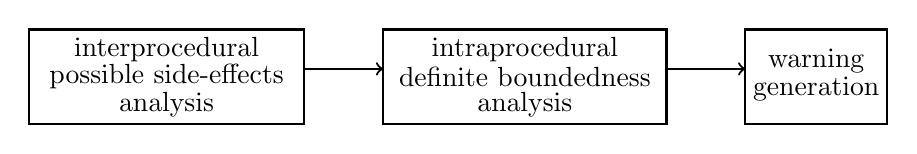
\begin{tikzpicture}
    \draw [thick] (-0.5,0) rectangle +(3.5,1.2);
    \draw (1.25,0.95) node{interprocedural};
    \draw (1.25,0.6) node{possible side-effects};
    \draw (1.25,0.25) node{analysis};

    \draw[->,thick] (3,0.7) -- +(1,0);

    \draw [thick] (4,0) rectangle +(3.6,1.2);
    \draw (5.8,0.95) node{intraprocedural};
    \draw (5.8,0.6) node{definite boundedness};
    \draw (5.8,0.25) node{analysis};

    \draw[->,thick] (7.6,0.7) -- +(1,0);

    \draw [thick] (8.6,0) rectangle +(1.8,1.2);
    \draw (9.5,0.8) node{warning};
    \draw (9.5,0.45) node{generation};
  \end{tikzpicture}
  \end{center}

\end{frame}

\begin{frame}\frametitle{Possible side-effects analysis}

  \begin{mdframed}[backgroundcolor=blue!20] 
  Goal: infer the elements type of the lists that might be enlarged
  during the execution of a piece of code
  \end{mdframed}

  \mbox{}\\

  It is the fixpoint $\intsideeffect$ of a bottom-up denotational abstract interpretation of execution traces:

  {\scriptsize
  \begin{align*}
      \sideeffect{c}=\sideeffect{v}&=\sideeffect{\nop}=\sideeffect{\return}=\varnothing\\
      \sideeffect{\push{\exp_1}{\exp_2}}&=\sideeffect{\exp_1}\cup\sideeffect{\exp_2}\cup
      \{t\mid\exp_1\text{ has type }\<List<>t\<\text{>}>\}\\
      \sideeffect{\new{C}{\exp_1,\ldots,\exp_n}}&=\intsideeffect(C.C)\cup\bigcup_{i=1}^n\sideeffect{\exp_i}\\
      \sideeffect{\call{\exp_0}{m}{\exp_1,\ldots,\exp_n}}&=\bigcup_{j=1}^k\intsideeffect(C_j.m)\cup\bigcup_{i=0}^n\sideeffect{\exp_i}\\
      \noalign{\centering\text{where $C_1.m\cdots C_k.m$ are the methods possibly called here}}
      \sideeffect{\ifetwo{\exp_1}{\exp_2}{\com_1}{\com_2}}&=\sideeffect{\exp_1}\cup\sideeffect{\exp_2}\cup\sideeffect{\com_1}\cup\sideeffect{\com_2}.
  \end{align*}
  }

\end{frame}

\begin{frame}[fragile]{Example: side-effect analysis of the gradual Ponzi scheme}

  \begin{center}
    \begin{minipage}{0.95\textwidth}
      \begin{lstlisting}[language=pseudo]
public class Ponzi1 extends Contract {
  private final List<Contract> investors;
  private int minimum_investment;

  public Ponzi1() {
    investors = new List();
    investors.push(caller);
    minimum_investment = 1000;
  }

  public payable void invest() {
    require(amount >= minimum_investment, "too little");

    int eachInvestorGets = amount / investors.size();
    for investor in investors
      investor.receive(eachInvestorGets);

    investors.push(caller);
    minimum_investment = amount * 11 / 10;
  }
}
      \end{lstlisting}
    \end{minipage}
  \end{center}

  \vspace*{-3ex}
  \[\intsideeffect(\<Ponzi1.Ponzi1>)=\{\<Contract>\}\qquad\intsideeffect(\<Ponzi1.invest>)=\{\<Contract>\}\]

\end{frame}

\begin{frame}[t]\frametitle{Definite boundedness analysis}

  \begin{mdframed}[backgroundcolor=blue!20] 
    Goal: infer definite upper bounds of the size of some path expressions
    referring to lists, against constants: $\size{\underbrace{\<v.f.g>}_{\|path\ \pi|}}\le\underbrace{100}_{\in\mathbb{N}}$.
  \end{mdframed}

  \mbox{}\\

  \only<1>{
  It is a small step abstract operational semantics over pairs
  \[
  \langle\text{program point},\text{set of upper bounds}\rangle
  \]
  }

  \only<2>{
    \[\frac{\Pi(p)=\nop}
         {\pair{p}{\|bo|}\boderivation\pair{p_{\|next|}}{\|bo|}}\]
  }

  \only<3>{
    \[\frac{\Pi(p)=(\assign{\lvalue}{\exp})\quad\pair{\lvalue}{\|bo|}\boderivation\|bo|'\quad\pair{\exp}{\|bo|'}\boderivation\|bo|''}
           {\pair{p}{\|bo|}\boderivation\pair{p_{\|next|}}{\|assign|(\|bo|'',\assign{\lvalue}{\exp})}}\]
  \vspace*{-2ex}
  \begin{align*}
    \|assign|(\|bo|,\assign{\pi}{\new{\mathtt{List}}{}})&=\|bo|^{-\pi}\cup\{\size{\pi}\le 0\}\\
    \|assign|(\|bo|,\assign{\pi}{\pi'})&=\|bo|^{-\pi}\cup\{\size{\pi}\le n\mid(\size{\pi'}\le n)\in\|bo|\}\\
    \|assign|(\|bo|,\assign{\pi}{\exp})&=\|bo|^{-\pi}\text{ in all other cases not considered above}\\
    \|assign|(\|bo|,\assign{\lvalue}{\exp})&=\|bo|\text{ if $\lvalue$ is not a path}
  \end{align*}
  }

  \only<4>{
    \[
    \frac{\Pi(p)=(\receive{\exp_1}{\exp_2})\quad\pair{\exp_1}{\|bo|}\boderivation\|bo|'\quad\pair{\exp_2}{\|bo|'}\boderivation\|bo|''}
         {\pair{p}{\|bo|}\boderivation\pair{p_{\|next|}}{\|bo|''}}
    \]
  }

  \only<5>{
    \[
    \frac{\begin{array}{c}
        \Pi(p)=(\push{\exp_1}{\exp_2})\quad\pair{\exp_1}{\|bo|}\boderivation\|bo|'\quad\pair{\exp_2}{\|bo|'}\boderivation\|bo|''\\
        \exp_1\text{ has type \<List<$t$\texttt{>}>}\\
        \|bo|_{\text{survives}}=\left\{(\size{\pi}\le n)\in\|bo|''\left|\begin{array}{l}\pi\text{ survives if a list}\\
        \text{of $t$ gets enlarged}\end{array}\right.\right\}\\
        \|bo|_{\neg\text{survives}}=\left\{\size{\pi}\le n+1\left|\begin{array}{l}
        (\size{\pi}\le n)\in\|bo|''\text{ and}\\
        \pi\text{ might not survive if a list}\\
        \text{of $t$ gets enlarged}
        \end{array}\right.\right\}
    \end{array}}
         {\pair{p}{\|bo|}\boderivation\pair{p_{\|next|}}{\|bo|_{\text{survives}}\cup\|bo|_{\neg\text{survives}}}}
    \]
  }

  \only<6>{
    \[
    \frac{\Pi(p)=\left(\ifetwo{\exp_1}{\exp_2}{\com_{\|then|}}{\com_{\|else|}}\right)\quad
      \begin{array}{c}
        \pair{\exp_1}{\|bo|}\boderivation\|bo|'\\
        \pair{\exp_2}{\|bo|'}\boderivation\|bo|''
      \end{array}}
         {\pair{p}{\|bo|}\boderivation\pair{p_{\|then|}}{\|bo|''}}\]
  }

  \only<7>{
    \vspace*{-4.5ex}
    \[
    \frac{\Pi(p)=\left(\ifetwo{\exp_1}{\exp_2}{\com_{\|then|}}{\com_{\|else|}}\right)\quad
      \begin{array}{c}
        \pair{\exp_1}{\|bo|}\boderivation\|bo|'\\
        \pair{\exp_2}{\|bo|'}\boderivation\|bo|''
      \end{array}}
         {\pair{p}{\|bo|}\boderivation\pair{p_{\|then|}}{\|improve|(\|bo|'',\cop{\exp_1}{\exp_2})}}\]
  \vspace*{-2ex}
  \begin{align*}
    \|improve|(\|bo|,\copfull{\size{\pi}}{\le}{n})&=\|bo|\cup\{\size{\pi}\le n\}\\
    \|improve|(\|bo|,\copfull{\size{\pi}}{<}{n})&=\|bo|\cup\{\size{\pi}\le n-1\}\\
    \|improve|(\|bo|,\copfull{n}{\ge}{\size{\pi}})&=\|bo|\cup\{\size{\pi}\le n\}\\
    \|improve|(\|bo|,\copfull{n}{>}{\size{\pi}})&=\|bo|\cup\{\size{\pi}\le n-1\}\\
    \|improve|(\|bo|,\cop{\exp_1}{\exp_2})&=\|bo|\text{ in all other cases}
  \end{align*}
  }

  \only<8>{
    \[\frac{\begin{array}{c}
        \Pi(p)=(\call{\exp_0}{m}{\exp_1,\ldots,\exp_p})\\
        \pair{\exp_0}{\|bo|}\boderivation\|bo|_0\quad\cdots\quad\pair{\exp_p}{\|bo|_{p-1}}\boderivation\|bo|_p\\
        \text{$C_1.m\cdots C_k.m$ are the methods possibly called here}\\
        \|bo|'=\left\{(\size{\pi}\le n)\in\|bo|_p\left|\begin{array}{l}
        \pi\text{ survives if a list of}\\
        \cup_{i=1}^k{\color{blue}\intsideeffect}(C_i.m)\text{ gets enlarged}
        \end{array}\right.\right\}
    \end{array}}{\pair{p}{\|bo|}\boderivation\pair{p_{\|next|}}{\|bo|'}}\]
    \begin{center}
      {\color{blue}note the use of the side-effect analysis $\intsideeffect$ computed before}
    \end{center}
  }

\end{frame}

\begin{frame}\frametitle{Computation of the abstract semantics for boundedness}

  \begin{itemize}
  \item The analysis starts at the beginning of the methods, with the $\varnothing$ approximation
    (\ieinitial nothing is known at the beginning of a method)
  \item The small step operational semantics is propagated from there along all possible execution paths
  \item When passing twice from the same program point, the least upper bound of the old and new approximations
    is used to continue the propagation
  \item Our abstract domain has infinite ascending chains: a widening is used to ensure termination
    in case of loops
  \end{itemize}

\end{frame}

\begin{frame}[fragile]\frametitle{The boundedness analysis of the Ponzi scheme}

  \begin{lstlisting}[language=pseudo,numbers=none]
  public Ponzi1() {
    |\invariant{$\varnothing$}|
    investors = new List();
    |\invariant{$\{\size{\mathtt{this.investors}}\le 0\}$}|
    investors.push(caller);
    |\invariant{$\{\size{\mathtt{this.investors}}\le 1\}$}|
    minimum_investment = 1000;
  }

  public payable void invest() {
    |\invariant{$\varnothing$}|
    require(amount >= minimum_investment, "too little");
    |\invariant{$\varnothing$}|
    int eachInvestorGets = amount / investors.size();
    |\invariant{$\varnothing$}|
    for investor in investors
      |\invariant{$\varnothing$}|
      investor.receive(eachInvestorGets);
    |\invariant{$\varnothing$}|
    investors.push(caller);
    |\invariant{$\varnothing$}|
    minimum_investment = amount * 11 / 10;
  }
  \end{lstlisting}

\end{frame}

\begin{frame}[fragile]\frametitle{The boundedness analysis of the fixed Ponzi scheme}

  \begin{lstlisting}[language=pseudo,numbers=none]
  public Ponzi2() {
    [ identical as in Ponzi1 ]  
  }

  public payable void invest() {
    |\invariant{$\varnothing$}|
    require(amount >= minimum_investment, "too little");
    |\invariant{$\varnothing$}|
    while (investors.size() > 100)
      |\invariant{$\varnothing$}|
      investors.removeFirst();
    |\invariant{$\{\size{\mathtt{this.investors}}\le 100\}$}|
    int eachInvestorGets = amount / investors.size();
    |\invariant{$\{\size{\mathtt{this.investors}}\le 100\}$}|
    for investor in investors
      |\invariant{$\{\size{\mathtt{this.investors}}\le 100\}$}|
      investor.receive(eachInvestorGets);
    |\invariant{$\{\size{\mathtt{this.investors}}\le 100\}$}|
    investors.push(caller);
    |\invariant{$\{\size{\mathtt{this.investors}}\le 101\}$}|
    minimum_investment = amount * 11 / 10;
  }
  \end{lstlisting}
\end{frame}

\begin{frame}[fragile]\frametitle{The boundedness analysis of the lottery example}
  \begin{lstlisting}[language=pseudo,numbers=none]
  public payable void buy() {
    |\invariant{$\varnothing$}|
    Round last = rounds.last();
    |\invariant{$\varnothing$}|
    if (now > last.endTime) {
      |\invariant{$\varnothing$}|
      last = new Round(now + duration);
      |\invariant{$\{\size{\mathtt{last.sales}}\le 0\}$}|
      rounds.push(last);
      |\invariant{$\{\size{\mathtt{last.sales}}\le 0\}$}|
    }
    else {
      |\invariant{$\varnothing$}|
      nop;
      |\invariant{$\varnothing$}|
    }

    |\invariant{$\varnothing$}|
    last.sales.push(...);
    |\invariant{$\varnothing$}|
  }
  \end{lstlisting}
\end{frame}

\begin{frame}[fragile]\frametitle{The boundedness analysis of the fixed lottery example}
  \begin{lstlisting}[language=pseudo,numbers=none]
  public payable void buy() {
    |\invariant{$\varnothing$}|
    Round last = rounds.last();
    |\invariant{$\varnothing$}|
    if (now > last.endTime or last.sales.size() >= 5000) {
      |\invariant{$\varnothing$}|
      last = new Round(now + duration);
      |\invariant{$\{\size{\mathtt{last.sales}}\le 0\}$}|
      rounds.push(last);
      |\invariant{$\{\size{\mathtt{last.sales}}\le 0\}$}|
    }
    else {
      |\invariant{$\{\size{\mathtt{last.sales}}<=4999\}$}|
      nop;
      |\invariant{$\{\size{\mathtt{last.sales}}<=4999\}$}|
    }

    |\invariant{$\{\size{\mathtt{last.sales}}<=4999\}$}|
    last.sales.push(...);
    |\invariant{$\{\size{\mathtt{last.sales}}<=5000\}$}|
  }
  \end{lstlisting}
\end{frame}

\begin{frame}\frametitle{Warning generation}

  All lists of type $t$ are \emph{bounded}
  if for every $\push{\exp_1}{\exp_2}$ in the program such that
  $\<List<$t'$\texttt{>}>$ is the type of $\exp_1$,
  $t$ and $t'$ share a subtype and $\|bo|$ is the boundedness computed
  at the \<push>, it is
  \begin{enumerate}
  \item $\exp_1=\pi$ is a path
  \item $(\size{\pi}\le n)\in\|bo|$ for some $n\in\nat$
  \end{enumerate}

  \medskip

  \begin{mdframed}[backgroundcolor=blue!20] 
  Our analyzer issues a warning at each
  \[
  \for{v}{\exp}{\com}
  \]
  in the program, where
  $\exp$ has type $\<List<$t$\texttt{>}>$, if and only if it is not true that
  all lists of type $t$ are bounded
  \end{mdframed}
  
\end{frame}

\begin{frame}\frametitle{Results}

  \begin{center}
  \begin{tabular}{|c|c|c|}
    \hline
    smart contract & expected & actual \\\hline\hline
    \<Ponzi1> & warning & warning \\\hline
    \<Ponzi2> & no warning & no warning \\\hline
    \<Lottery1> & warning & warning \\\hline
    \<Lottery2> & no warning & no warning\\\hline
  \end{tabular}
  \end{center}

  \bigskip

  Try it yourself in our repository:

  \begin{mdframed}[backgroundcolor=blue!20] 
  \<mvn clean test -Dtest=Ponzi1Tests -Dprint>

  \<mvn clean test -Dtest=Ponzi2Tests -Dprint>

  \<mvn clean test -Dtest=Lottery1Tests -Dprint>

  \<mvn clean test -Dtest=Lottery2Tests -Dprint>
  \end{mdframed}

\end{frame}

\begin{frame}[fragile]\frametitle{Imprecision: \<if> instead of \<while>}

  \begin{center}
    Static analysis must be imprecise because it tackles undecidable properties
  \end{center}

  \vspace*{-1.5ex}
  \begin{center}
    \begin{minipage}{0.95\textwidth}
      \begin{lstlisting}[language=pseudo]
public class Ponzi3 extends Contract {
  private final List<Contract> investors;
  private int minimum_investment;

  public Ponzi3() { ... }

  public payable void invest() {
    require(amount >= minimum_investment, "too little");

    [correct fix but the analyzer issues a false warning here]
    if (investors.size() > 100)
      investors.removeFirst();

    int eachInvestorGets = amount / investors.size();
    for investor in investors
      investor.receive(eachInvestorGets);

    investors.push(caller);
    minimum_investment = amount * 11 / 10;
  }
}
      \end{lstlisting}
    \end{minipage}
  \end{center}

\end{frame}

\begin{frame}\frametitle{Conclusion}

  A specialized analysis for a real problem of smart contracts
  \begin{itemize}
  \item simpler and faster than more general computations of data size
    (polyhedra): a comparison in ongoing
  \item able to reason about size of fields of fields\ldots
  \item implemented on a toy language
  \item paper in advanced preparation for a conference
  \end{itemize}
\end{frame}

\end{document}
